\subsection{Exemples d'application}
\begin{UPSTIactivite}[2][Salle de classe][][\,][Exemple]
	\begin{center}
		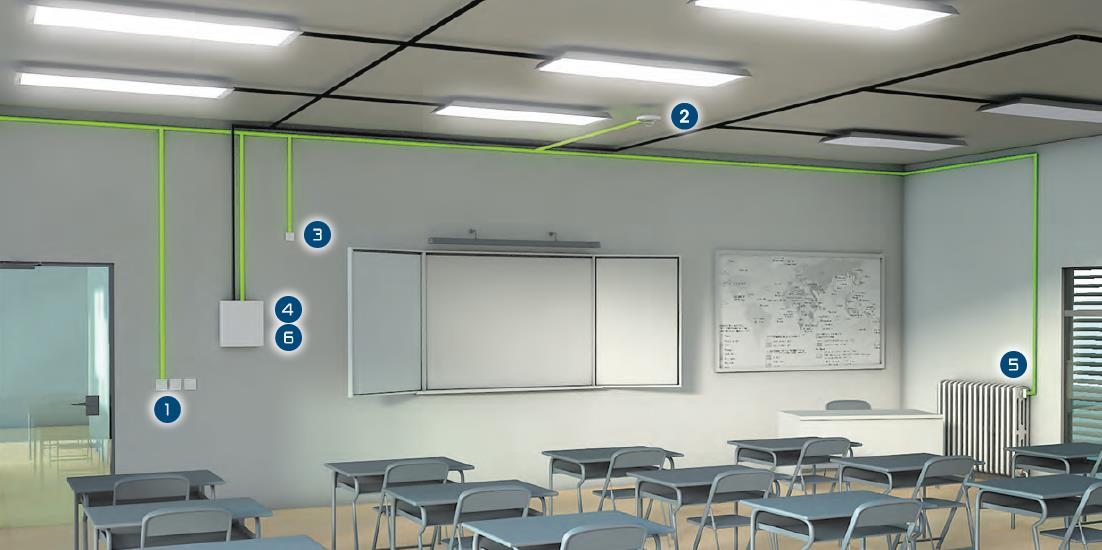
\includegraphics[width=.9\linewidth]{salleClasse}
	\end{center}
    \begin{multicols}{3}
		\begin{itemize}[label=\dots]
			\item Capteur de CO2
			\item Détecteur de présence
			\item Interrupteurs
			\item Variateur d'éclairage DALI
			\item Régulateur de chauffage
			\item Commande de store KNX
		\end{itemize}
	\end{multicols}
    \UPSTIquestion{Associer un élément à chaque numéro sur le schéma.}
    \UPSTIquestion{Pour chacun, indiquer s'il s'agit d'un capteur, ou d'un actionneur.}
\end{UPSTIactivite}

\begin{UPSTIactivite}[2][Salle industrielle][][\,][Exemple]
	\begin{center}
		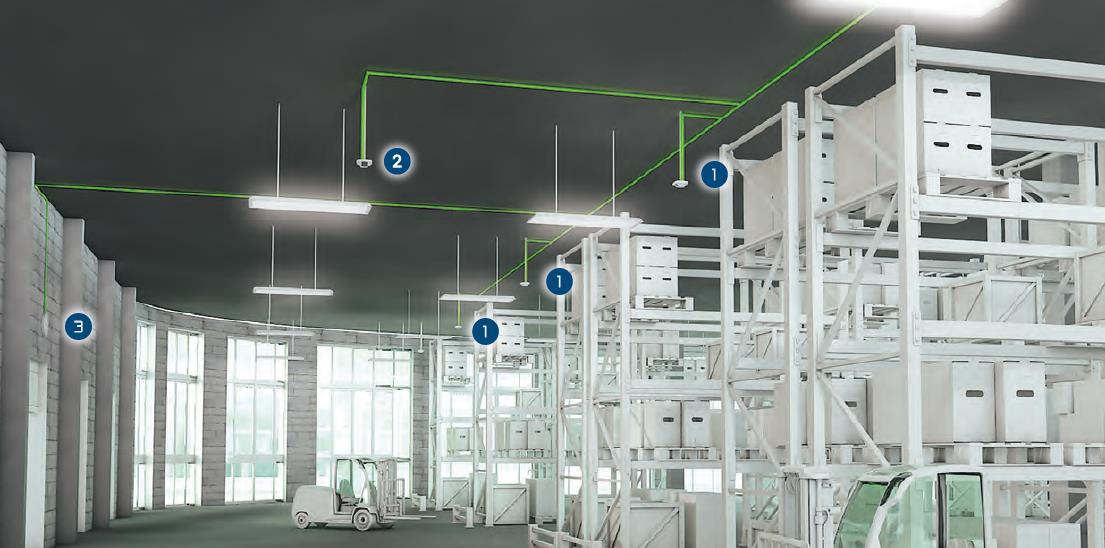
\includegraphics[width=.9\linewidth]{industrie}
	\end{center}
    \begin{multicols}{3}
		\begin{enumerate}
			\item Détecteur présence rayon
			\item Détecteur présence circulation
			\item Commande DALI
		\end{enumerate}
	\end{multicols}
\end{UPSTIactivite}

\begin{UPSTIactivite}[2][Bâtiment non résidentiel][][\,][Exemple]
	\begin{center}
		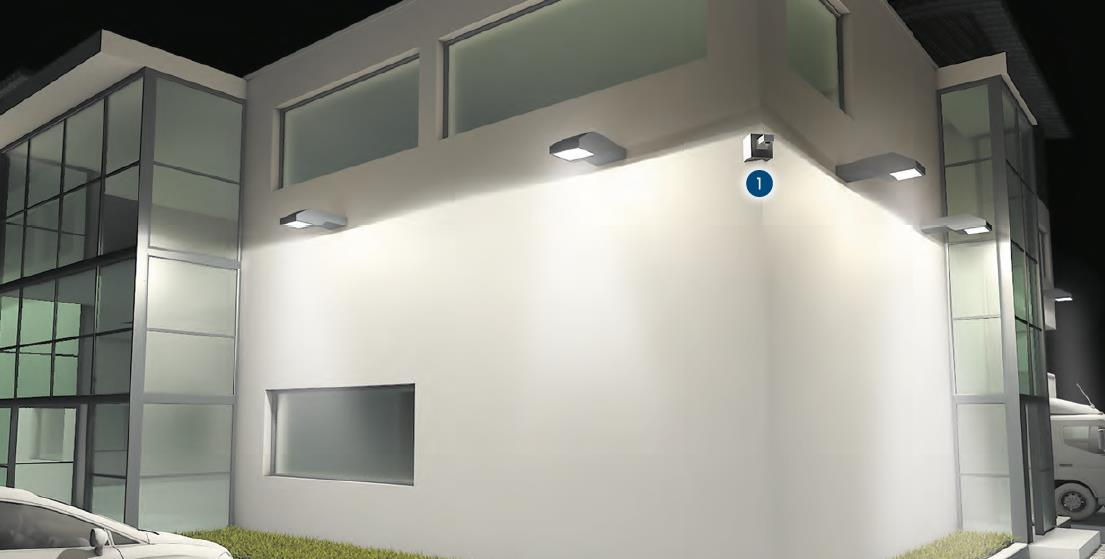
\includegraphics[width=\linewidth]{nonResidentiel}
	\end{center}
    \begin{multicols}{3}
		\begin{itemize}
			\item Détecteur de mouvement
			\item Capteur de luminosité
			\item Capteur de pluie
			\item Anémomètre
			\item Actionneur de store
			\item Alarmes
		\end{itemize}
	\end{multicols}
\end{UPSTIactivite}

\begin{UPSTIactivite}[2][Bâtiment résidentiel][][\,][Exemple]
	\begin{center}
		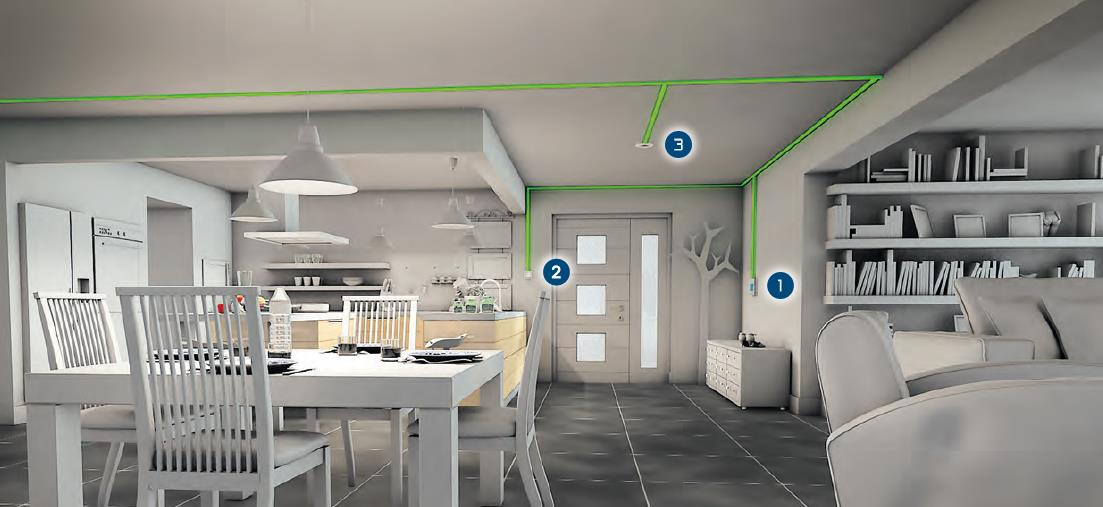
\includegraphics[width=\linewidth]{residentiel}
	\end{center}
    \begin{multicols}{2}
		\begin{enumerate}
			\item Écran multifonction 
            \item Module d'entrée (Boutons, interrupteurs)
			\item Détecteur de présence
			\item Actionneurs commutateurs
			\item etc. 
		\end{enumerate}
	\end{multicols}
\end{UPSTIactivite}


